
\documentclass[brazilian,12pt,a4paper,final]{article}


\usepackage[a4paper,
bindingoffset=0.2in,
left=0.8in,
right=0.8in,
top=0.8in,
bottom=0.8in,
footskip=.25in]{geometry}

%% Pacotes extras (opcionais):

% *babel* contem as regras de hifenização
\usepackage[portuguese]{babel}
% *t1enc* permite o reconhecimento dos acentos inseridos com o teclado
\usepackage{t1enc}

% *inputenc* com opção *utf8* permite reconhecimento dos caracteres com codificação UTF8, que é padrão dos esditores de texto no Linux. Isso permite reconhecimento automático de acentuação.
%\usepackage[utf8]{inputenc}
\usepackage{epsfig}

% *graphicx* é para incluir figuras em formato eps 
\usepackage{graphicx} % para produzir PDF diretamente reescrever esta linha assim: \usepackage[pdftex]{graphicx}

% *color* fontes soloridas
\usepackage{color}
%%% fim do cabecalho %%%

\pagestyle{empty}
\title{Métodos Computacionais Aplicados à Biocomplexidade}
\author{Aluno: André Gustavo Dessoy Hubner - Matrícula: 00315569 \\ IF-UFRGS}

\begin{document}
	\maketitle
	
	\section{Introdu\c{c}\~ao} 
	% Aqui a Introdução \c{c} e \~a  é a forma standar  de escrever
	% carateres ASCII extendidos (acentos, etc), porem com o pacote t1enc
	% declarado acima podemos escrever diretamente ç em lugar d \c{c}, etc
	\indent 
	Esta tarefa tem como objetivo estudar a criação de uma árvore filogenética a partir de alinhamentos múltiplos e uma implementação do algoritmo de Kruskal a partir de um programa construído em Python e com a biblioteca Biopython.
	
	\section{Metodologia}
	\subsection{Busca de genes de rRNA 16S}
	O primeiro passo na construção da árvore foi buscar por genes de RNA ribossômico 16S de pelo menos 10 espécies devido ao seu já bem estabelecido potencial em explicitar as relações filogenéticas entre os organismos com base na evolução de sua sequência. Esta busca foi construída de forma semelhante a tarefas passadas, utilizando o módulo "Entrez" do Biopython para primeiro realizar a busca como seria feito no site do NCBI com a função "esearch" e depois conseguir as sequências de fato com "efetch".
	\vspace{0.5cm}
	
	Mais detalhadamente, na primeira função buscamos no banco de dados "nucleotide" pelo termo "16S ribosomal RNA gene[Titl] NOT partial sequence[Titl] NOT uncultured[Titl] NOT clone[Titl]", que essencialmente retornará sequências quaisquer de gene de RNA ribossômico 16S que não sejam alguns tipos de sequência incompleta, obtendo assim sequências de boa qualidade, e retornando 100 resultados ao especificar o parâmetro "retmax" com o valor de 100.
	\vspace{0.5cm}
	
	Com os resultados dessa busca obteve-se então uma lista dos ids dos resultados, que para adicionar um elemento de aleatoriedade, foi submetida ao método "sample" da biblioteca "random". Esta função irá fazer, bem como diz seu nome, uma amostragem da lista passada de acordo com o valor k passado, que foi escolhido como 10 aqui. Esta lista amostrada é então passada ao efetch, buscando também em nucleotide e especificando o tipo de retorno como "fasta", retornando finalmente as sequências desejadas. Após um leve uso de manipulação de strings básica de Python, elas estão prontas para serem alinhadas entre si.
	\vspace{0.5cm}
	
	\subsection{Alinhamento múltiplo e matriz de distância}
	
	Para o alinhamento múltiplo global, foi utilizado o módulo Align do Biopython. Embora tenha sido instruída a utilização do módulo pairwise2, esta dependência está marcada como obsoleta pela própria equipe do Biopython em sua documentação, e sua usabilidade é bem pior do que a das funcionalidades usadas aqui. Ainda assim, tentou-se primeiramente ela, no entanto ficou claro rapidamente que suas funções de alinhamento  necessariamente tomavam um tempo muito grande e pareciam alinhar várias vezes para apenas um alinhamento específicado, retornando o mesmo score para todos. A utilização do módulo Align pareceu não só melhor como ter resultados mais confiáveis, depois de verificar ambas as opções.
	\vspace{0.5cm}
	
	Apenas duas funcionalidades do Align foram necessárias aqui, sendo estas a classe "PairwiseAligner" e o método score() de objetos dessa classe. Através do primeiro, pode-se criar um objeto para realizar alinhamentos com grande capacidade e facilidade de customização, podendo especificar os valores de score a serem atribuídos a virtualmente cada situação. Neste projeto foi criada uma instância utilizando valores de match como 5, mismatch como -4, gap -10 e extensão de gap -1, além de especificar a realização de alinhamentos globais. Assim, utilizando dois laços de repetição, um aninhado no outro, foi possível usar o score() para realizar o alinhamento entre cada sequência das 10 anteriores, retornando apenas a informação que seria utilizada posteriormente, o score de cada alinhamento. 	
	\vspace{0.5cm}
	
	Esses scores, cada um informando a pontuação do alinhamento de uma das sequências com outra, foram armazenados em uma matriz de pontos utilizando listas de Python. Para transformar esta matriz em uma matriz de distâncias, precisava-se ainda aplicar um processamento para cada valor, de acordo com as seguintes regras: 
	\begin{itemize}
		\item Se ele fosse igual a zero, significava que era um alinhamento entre as mesmas sequências (nas iterações anteriores se aplicou a lógica para retornar 0 caso fossem as mesmas sequências), e então se retorna zero. 
		\item Se fosse menor que zero, significava um score negativo (ou seja, fraco), portanto seria necessário convertê-lo a um valor grande, representando uma grande distância. Isto foi feito simplesmente invertendo o sinal do resultado.
		\item Não sendo nenhum dos dois, eleva-se o valor a -1, resultando em números positivos tão menores quanto o valor original era grande.
	\end{itemize}
	\vspace{0.5cm}
	
	Foi feita ainda uma função simples para visualizar as duas matrizes geradas. As figuras 1 e 2 mostram esse resultado para as matrizes de pontos e de distância, respectivamente. As matrizes expostas não são dos mesmos dados usados para figuras posteriores devido à aleatoriedade garantida por execução do programa, no entanto são representativas do padrão de sequências que são obtidas.
\left( 
	
	\begin{figure}[hbtp]
		\begin{center}
			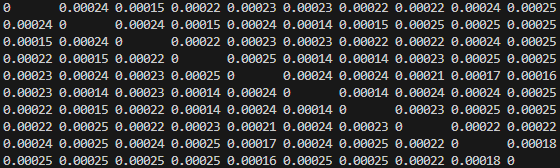
\includegraphics[]{matrizDistancia.png}
			\caption{Matriz de distâncias obtida a partir de um processamento adicional da matriz anterior.}
			\label{fig}
		\end{center}
	\end{figure}
	
	\subsection{Construção da árvore em formato Newick}
	
	Construída a matriz de distâncias, já se havia todos os dados necessários para construir a árvore filogenética. Já tinha sido mencionado que isto seria feito implementando o algoritmo de Kruskal, entretanto para realizar cada inserção dessa árvore, seria necessário realizá-la em uma string que pudesse ser representada como uma árvore filogenética. Para isso serve o padrão de representação Newick, que sendo o modelo mais simples e também um dos mais utilizados para representar árvores filogenéticas, foi o padrão escolhido nesta ocasião. 
	\vspace{0.5cm}
	
	A lógica começa na função BuildTree, que recebe a matriz de distâncias e uma lista de códigos dos organismos alvos e retorna a representação em string da árvore gerada. Após a inicialização de variáveis que serão utilizadas ao longa da execução, já será realizada a primeira varredura na matriz de distâncias buscando pelo menor valor. É importante notar aqui que embora a matriz gerada anteriormente seja simétrica, a busca será realizada em apenas um dos lados simétricos. Assim, após uma varredura total desse lado o menor valor encontrado será usado para unir as sequências dessa posição na matriz na etapa seguinte. A lógica desta execução está na função SearchMinimum, que retorna não só esse valor como os dois índices representando a posição das sequências da linha e da coluna, respectivamente. Ela está representada na figura 3.
	
	\begin{figure}[hbtp]
		\begin{center}
			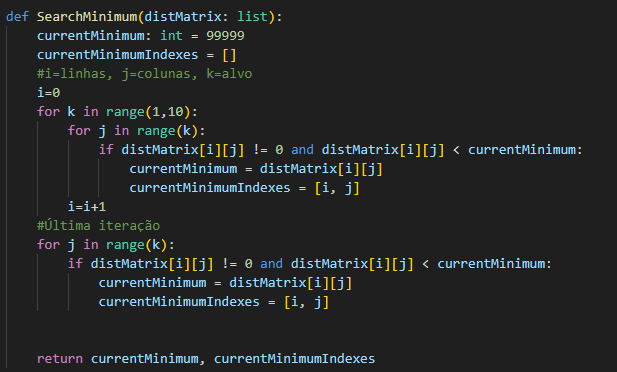
\includegraphics[]{SearchMinimum.png}
			\caption{Função que performa uma busca inteira por um dos lados da matriz pelo valor mínimo, retornando-o junto dos índices das sequências da linha e da coluna da posição.}
			\label{fig}
		\end{center}
	\end{figure}
	
	Logo após a execução dessa função a posição na qual foi obtida esse mínimo é modificada com o valor 99999, representando que aquela posição já foi usada. Inclusive antes mesmo desta modificação, é performada uma checagem de se o valor encontrado é igual a esse número, o que seria um dos pontos de retorno possíveis da árvore completa gerada. A figura 4 mostra a primeira execução dessa lógica.
	
	\begin{figure}[hbtp]
		\begin{center}
			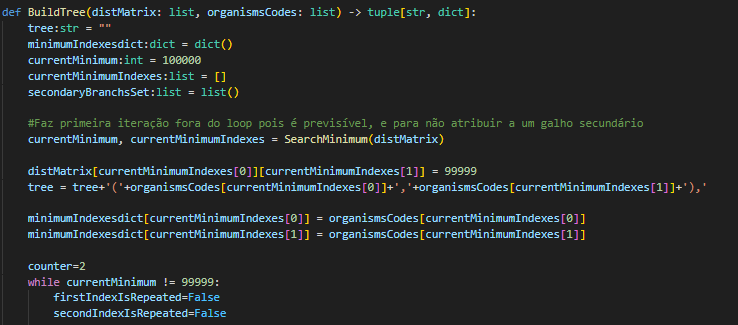
\includegraphics[width=15cm]{BuildTree.png}
			\caption{Função que performa uma busca inteira por um dos lados da matriz pelo valor mínimo, retornando-o junto dos índices das sequências da linha e da coluna da posição.}
			\label{fig}
		\end{center}
	\end{figure}
	
	Como é possível ver, temos as seguintes variáveis, junto de suas funções:
	\begin{itemize}
		\item tree: é a árvore sendo construída, crescendo a cada iteração. 
		\item minimumIndicesDict: serve para ter controle de quais índices (sequências) já foram adicionadas 
		à árvore.
		\item currentMinimum: receberá o valor mínimo encontrado em SeachMinimum; inicializada com 100000 para que qualquer valor encontrado seja menor.
		\item currentMinimumIndexes: índices dos mínimos encontrados na última execução de SearchMinimum; são adicionados em minimumIndexesDict logo após essa execução.
		\item secondaryBranchesSet: representa um conjunto de ramos (partes da árvore) que não fazem parte do ramo principal ainda, e que terão uma lógica de inserção diferente quando forem inseridos posteriormente.
	\end{itemize}
		
	O ramo secundário mencionado nesta última variável é uma limitação da abordagem utilizada aqui que precisa ser tratada, mas para entender sua função, primeiro é necessário saber mais da implementação do algoritmo usada aqui. De acordo com o algoritmo de Kruskal, cada vez que vai ser adicionado um dos nós representando o alinhamento de dois organismos à árvore, deve-se saber se nenhum ou um deles já está inserido na árvore. Se um já está, simplesmente formamos um clado entre o organismo que não está e todo o clado que contém o outro organismo que já estava na árvore. Entretanto, se ambos não estavam na árvore, forma-se primeiro apenas um clado entre esses dois.
	\vspace{0.5cm}
	
	 Como se sabe que todos os clados formados serão imediatamente ou eventualmente inseridos em um clado "principal" e que a lógica de inserção  desse último caso é diferente (são dois ou mais organismos sendo inseridos na árvore principal ao invés de um), primeiro é realizada uma iteração fora do laço de repetição para definir uma "árvore principal", e posteriormente todas as vezes que clados são formados desta forma eles são tratados como "galhos secundários", que apesar de serem imediatamente adicionados à árvore através do controle de "minimumIndicesDict", precisam de um controle adicional através de "secondaryBranchesSet" para realizar a lógica apropriada de inserção à árvore principal quando os índices do mínimo encontrado representarem um organismo já na árvore principal e outro em um "galho" secundário.
	 \vspace{0.5cm}
	 
	 A primeira execução mencionada é o que vemos na figura 4. A partir de então, começa um laço de repetição que só quebrará ao todos os organismos serem inseridos na árvore e nenhuma árvore secundária sobrar, ou o valor mínimo encontrado ser igual a 99999, o valor usado para descartar posições da matriz. Este último critério por sua vez nunca deve ser alcançado, uma vez que em toda iteração ocorre a inserção apropriada, e se não são atingidos os critérios para isso, verifica-se primeiro se o tamanho do dicionário de índices contém o mesmo número de elementos que o número de linhas na matriz e não há nada restando em galhos secundários, conforme explicado anteriormente, retornando então a árvore finalizada e terminando a execução de BuildTree caso essas condições sejam verdadeiras. O código com a lógica para qual tipo de modificação aplicar está demonstrado nas figuras 5 e 6.
	 \vspace{0.5cm}
	 
	 \begin{figure}[hbtp]
	 	\begin{center}
	 		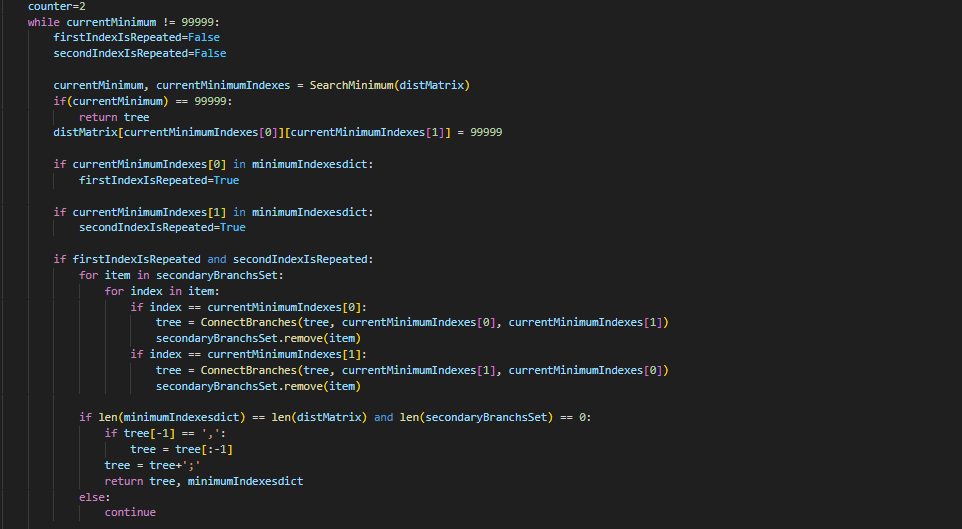
\includegraphics[]{FirstHalf.png}
	 		\caption{Primeira metade do código dentro do laço de repetição, contendo a lógica para
	 			verificar se vai haver uma inserção de um galho secundário na árvore principal e se a árvore está terminada.}
	 		\label{fig}
	 	\end{center}
	 \end{figure}
	 
	 \begin{figure}[hbtp]
	 	\begin{center}
	 		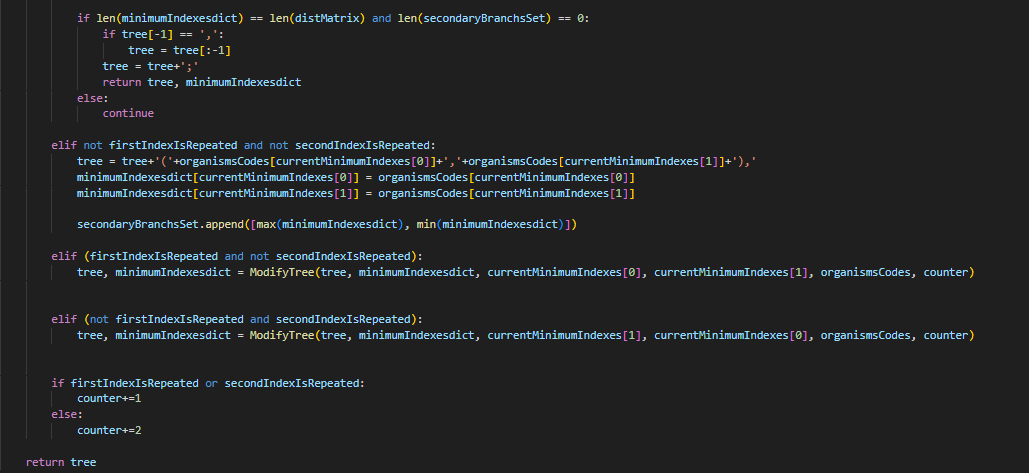
\includegraphics[]{SecondHalf.png}
	 		\caption{Segunda metade do código dentro do laço de repetição, contendo primero a condição de inserir uma galho secundário e depois os dois casos de inserção de um organismo à árvore principal.}
	 		\label{fig}
	 	\end{center}
	 \end{figure}
	 
	 Conforme é possível ver nas figuras, os códigos para inserir um galho secundário à árvore principal e apenas um organismo a ela estão encapsulado pelos métodos "ConnectBranches" e "ModifyTree", respectivamente, que foram omitidos aqui por envolverem muito mais questões técnicas do que algo que já não foi explicado do funcionamento do algoritmo.
	 Chegado o fim da função, temos por fim uma string representando uma árvore em formato Newick e seguindo a distância filogenética estimada de acordo com o algoritmo de Kruskal.
	 
	 \section{Resultados}
	 \subsection{Árvore gerada a partir do algoritmo e base de comparação}
	 
	 Ainda dentro do código, foram utilizadas duas funções do módulo Phylo do Biopython para validar e visualizar a árvore gerada, sendo estas a "draw\_ascii" e a "draw". No entanto, como ambas esperam um argumento no formato de árvore do mesmo módulo, a string da árvore foi primeiro convertida para um objeto StringIO através de conversão explícita direta, e logo depois para uma árvore do Biopython com Phylo.read(), passando a árvore e o formato "newick" como argumentos. A partir da variável resultante foi possível visualizar a árvore com ambas as funções draw, e o resultado da mais detalhada está na figura 7.
	 
	  \begin{figure}[hbtp]
	 	\begin{center}
	 		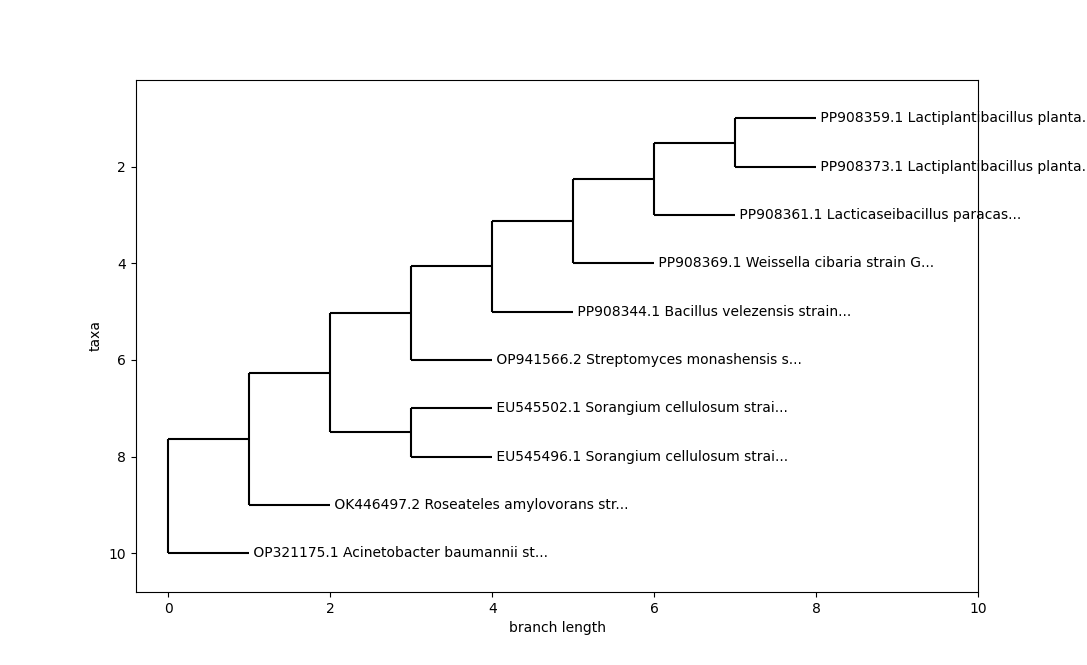
\includegraphics[width=15cm]{filogenia.png}
	 		\caption{Árvore filogenética resultante do algoritmo aplicado e de sua visualização através do método draw.}
	 		\label{fig}
	 	\end{center}
	 \end{figure}
	 
	 Nota-se que a visualização tem uma qualidade limitada, porém, na própria documentação do módulo há poucos detalhes sobre a configuração da chamada ao método draw. Como se sabe que essa função ,na verdade, usa funcionalidades da biblioteca Matplotlib, foi tentada uma configuração direta com esta, o que não foi bem sucedida. Apesar disso, a árvore gerada claramente tem a estrutura de uma árvore filogenética, assim como apresenta organismos de nomes semelhantes, classificados mais proximamentes na taxonomia, mais próximos um dos outros, o que é um indício visual claro de um bom resultado gerado.
	\vspace{0.5cm}
	 
	 
	 Todavia, para fazer reflexões relevantes sobre se a árvore gerada com este algoritmo é válida ou não, primeiro é necessário termos uma fonte de informação confiável sobre a distância filogenética dos organismos. Sendo assim, a partir de uma das execuções do código, foram coletados todos os códigos das sequências utilizadas na mesma execução, os quais foram então usados para gerar uma árvore filogenética com a ferramenta de árvore comum da seção de taxonomia do NCBI. Essa ferramenta estima as árvores puramente conforme as distâncias das classicações dos organismos, tal como informa sua página "help", logo, não subsitui análises filogenéticas minuciosas, mas usa uma base suficientemente credível.
	 \vspace{0.5cm}
	 
	  Ademais, como não é possível selecionar mais de um organismo de um mesmo tipo e há um número limitado de linhagens selecionáveis, a árvore gerada contém 10-N nós, em que N é o número de organismos da mesma espécie que vieram no resultado (aqui houve uma repetição de \textit{Sorangium cellulosum} e de \textit{Lactiplantibacillus plantarum}). A árvore resultante está disponível na figura 8.
	  
	  \begin{figure}[hbtp]
	  	\begin{center}
	  		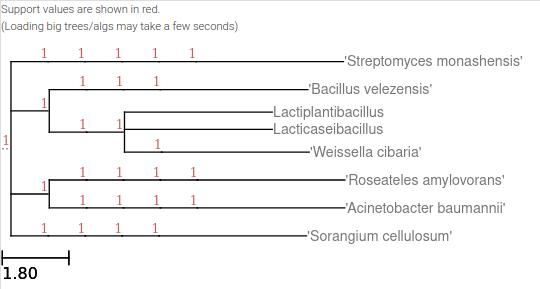
\includegraphics[]{Árvore NCBI.jpeg}
	  		\caption{Árvore obtida ao informar ao passar os mesmos organismos da execução do algoritmo de Kruskal à visualização de árvore comum do NCBI. Nota-se que há 8 nodos terminais ao invés de 10, devido a execução ter sorteado 10 organismos havendo duas repetições de espécie}
	  		\label{fig}
	  	\end{center}
	  \end{figure}
	 
	 	
	 \subsection{Comparação entre as duas árvores}
	 
	 Observando as duas árvores e considerando os nodos de \textit{Lactiplantibacillus plantarum} e de \textit{Sorangium cellulosum} na árvore externa como sendo na verdade um clado contendo as duas linhagens da mesma espécie conforme os dados da execução, são bastante notáveis alguns pontos positivos na árvore construída. Primeiramente, o caso mais óbvio é que tanto as repetições de \textit{Lactiplantibacillus plantarum} quanto de \textit{Sorangium cellulosum} estão mais próximas da sequência da outra linhagem da mesma espécie do que qualquer outra. O segundo ponto que é extremamente positivo é o fato de os dois \textit{Lactiplantibacillus plantarum}, o \textit{Lacticaseibacillus paracasei} e o \textit{Weissella cibaria}, todos estes pertencentes a gêneros da família \textit{Lactobacillaceae}, estarem mais próximos de si do que qualquer outro. E não só isso, como \textit{Bacillus velezensis}, que também é um bacilo, está mais próximo desses do que de outros. \textit{Roseateles amylovorans} e \textit{Acinetobacter baumannii}, pertencentes ao mesmo filo Pseudomonadota, também estão próximos.
	 \vspace{0.5cm}
	 
	 Por outro lado, o principal ponto negativo é o fato de que vários desses organismos deveriam estar no mesmo nível de hierarquia, conforme a árvore base. O clado representando todos os bacilos, por exemplo, está uma hierarquia abaixo de \textit{Streptomyces monashensis} e várias em relação aos outros, quando, na verdade, deveria estar no mesmo nível da árvore de acordo com a base (por todos serem bactérias). Outro caso disso é o fato de \textit{Roseateles amylovarans} estar um nível abaixo de \textit{Acinetobacter baumannii}, quando claramente ambas deveriam estar no mesmo nível, por ambos terem o mesmo filo em comum. Esta é sem dúvidas a principal limitação da abordagem utilizada aqui, o que limitaria bastante a utilização do algoritmo para gerar árvores úteis em maiores cenários. Um outro ponto negativo, de grau bem menor, porém, é que claramente o algoritmo utilizado não leva em conta as distâncias evolutivas para formar o tamanho dos galhos assim como é feito na árvore gerada pelo NCBI taxonomy, o que levaria um maior refinamento para implementar. 
	 \vspace{0.5cm}
	 
	 Resolvido o problema dos níveis da árvore, contudo, pelo menos com os dados obtidos aqui e com a observação rápida de outras execuções, sería um recurso muito útil para gerar árvores com o intuito de análisar as relações filogenéticas entre os organismos de uma forma mais geral, agrupando organismos semelhantes geneticamente mais perto um do outro através de suas sequências de gene de RNA 16S. Na implementação atual já é bem clara, após uma observação maior da árvore, o padrão com que ele forma as relações entre os organismos mais próximos, podendo ser útil para certas investigações mais rápidas.
	
	
\end{document}

